% Sections 10 to 12.

\section{Governance and Treasury}\label{sec:governance}

Power is separated into three chambers, each the guardian of one nature
of legitimacy. The miners, one computer one share of production, signal
protocol evolutions and keep the mining parameters: they embody security.
The Embers, one person one voice, vote budgets, identity rules and value
choices: they embody the community. High-Kleos identities arbitrate the
rules of the Ring, dispute precedents and reputation jurisprudence: they
embody memory. An ordinary change requires a majority in the two
concerned chambers; a constitutional modification, touching emission, the
Kleos layers or disclosure, requires all three. The separation is not
decorative: it reproduces, in protocol, the executive, legislative and
jurisdictional distinction that every democracy eventually discovered.

\begin{table}[htbp]
\centering
\small
\caption{Three legitimacies, three domains, no hidden passage.}
\label{tab:chambers}
\begin{tabularx}{\textwidth}{@{}L{2.3cm}YY@{}}
\toprule
Chamber & Composition and vote & Domain \\
\midrule
the miners & computing power produced (CPU), one vote per signed share of production & protocol, mining parameters, cadence \\
the Embers & one per person, non-biometric, one voice after deliberation & budgets, treasury, identity rules, values \\
the council of 70+ & identities with Kleos of at least 70, one vote per qualified identity & Ring rules, disputes, reputation precedents \\
\bottomrule
\end{tabularx}
\end{table}

The community treasury is the network's only levy: 6.18\,\% of block
rewards, a share chosen for recall, during the first eight eclipses,
thirty-two years. It is held in multisignature, spent by Ember vote,
published in full on chain, and extinguishes itself automatically at the
ninth eclipse: no tacit renewal, no fund of funds. The number is a
mnemonic; the structure is the argument: bounded in duration, budgeted in
public, spent by the community, dead by schedule. Its first charge is
engineering and audit; its second, once the Corona of
Section~\ref{sec:corona} activates its first working stage, is the
intelligence budget: senator salaries, red-team bounties and the
longevity bonuses are paid from a bounded slice of this same treasury,
never from a new emission channel. Development is explicitly funded,
because a zero-budget project is a dead project, but the resource belongs
to the community from the first block: no founder allocation, no
vesting, no investor. The fast governance track, for bounded parameters
such as base fees, remains subject to public delay and cancellation; the
constitutional track requires the three chambers and a six-month delay.
Nothing in that architecture can be changed behind the scenes: every
admission rule, every levy, every modification is a public transaction,
signed, archived for life.

\section{Monetary Design: The Golden Ratio Contract}\label{sec:economy}

The currency is called ATU. Its cap is 16,180,339 units, the golden
ratio multiplied by ten million, rounded to the integer. The choice of
symbol is an identity, and this version names it as such: the number is
a brand, chosen so the cap is exactly recitable, and it carries no
economic load. It is also a pleasant coincidence that RandomX, the
algorithm that will mine those units, seeds the same proportion in its
entrails: the constant \texttt{0x9E3779B9}, the integer truncation of the
golden ratio in binary arithmetic, drives the generation of its
superscalar programs. A contract one can recite from memory, to within
one digit, in ten years: sixteen million, the golden ratio, RandomX.
\begin{equation}\label{eq:phi}
\varphi = \frac{1 + \sqrt{5}}{2} \approx 1.618034,
\qquad
N = \left\lfloor \varphi \times 10^{7} \right\rfloor = 16{,}180{,}339 \text{ ATU}
\end{equation}

Emission follows a golden decay at the tempo of a century. Each eclipse,
four years and eight eras, emits 61.8\,\% of the previous one, that is,
the fraction $1/\varphi$. The first mints 6,180,340 ATU, the second
3,819,660, and their sum equals exactly ten million: 61.8\,\% of the
cap, the golden cut obtained with the round-number yardstick. The series
continues for thirty-four eclipses, the last absorbing the exact
remainder; 99\,\% of the mass exists around year forty, 99.9\,\% around
year sixty, and the ledger closes exactly at the cap in year 136. The
tempo is deliberately Bitcoin's, one easing every four years, because
four years is a proven social rhythm for a monetary calendar; the
proportion remained golden, 38.2\,\%, because it slows the decay gently
enough that every generation of miners finds an active emission. Those
are the functional reasons; the golden framing around them is the
network's identity, kept because a contract people can recite is a
contract people trust, and dropped nowhere else.
\begin{equation}\label{eq:eclipse}
E_k = \left\lfloor E_0 \cdot \varphi^{-k} \right\rfloor,
\qquad E_0 = 6{,}180{,}340 \text{ ATU}
\end{equation}
\begin{equation}\label{eq:cumulative}
S_n = \varphi^{2} \, E_0 \left( 1 - \varphi^{-n} \right),
\qquad S_2 = 10{,}000{,}000 \text{ exactly}
\end{equation}

\begin{figure}[htbp]
\centering
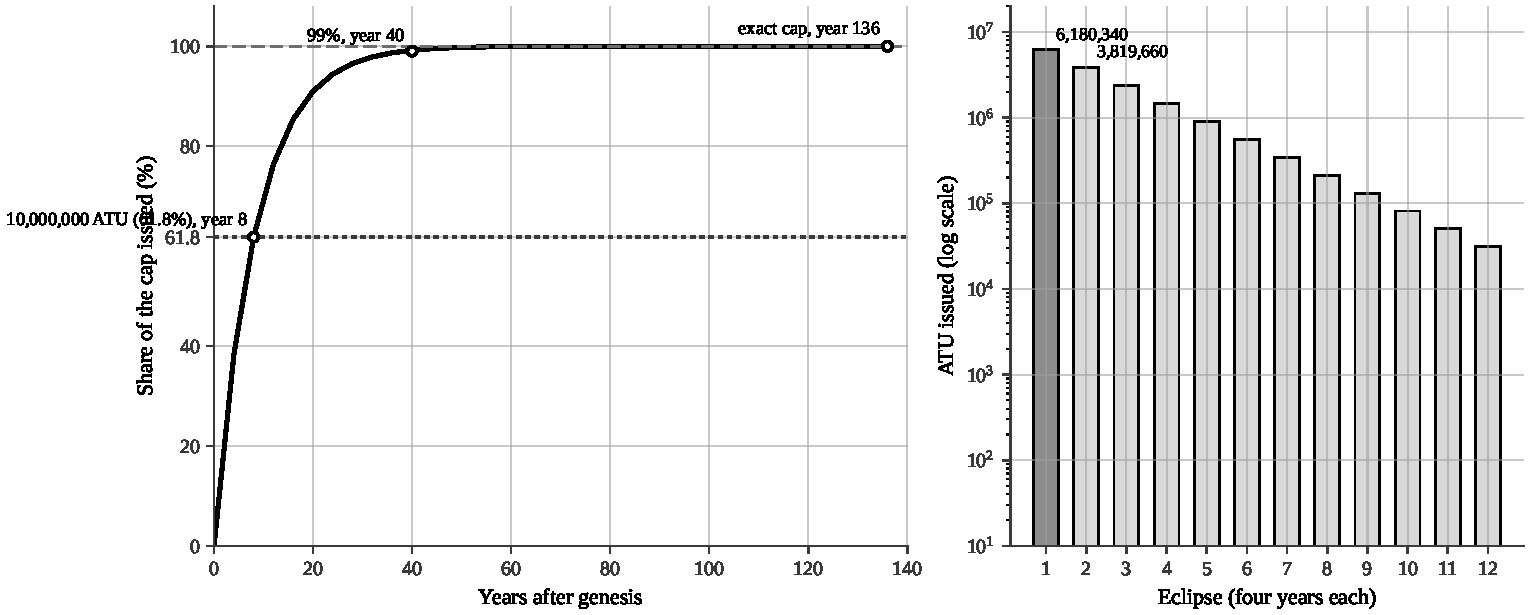
\includegraphics[width=0.96\textwidth]{wp-en-emission.pdf}
\caption{Cumulative emission toward the 16,180,339 ATU cap, and emission
per eclipse. The geometric series of ratio $1/\varphi$ closes the ledger
exactly at year 136.}
\label{fig:emission}
\end{figure}

\begin{table}[htbp]
\centering
\small
\caption{Golden eclipses: 34 eclipses, exact cap at year 136. Eclipses
not listed follow the same law.}
\label{tab:eclipses}
\begin{tabular}{@{}rrrrr@{}}
\toprule
Eclipse & Year & Emission (ATU) & Cumulative (ATU) & Share of cap \\
\midrule
1st & 4 & 6,180,340 & 6,180,340 & 38.2\,\% \\
2nd & 8 & 3,819,660 & 10,000,000 & 61.8\,\% \\
3rd & 12 & 2,360,679 & 12,360,679 & 76.4\,\% \\
4th & 16 & 1,458,980 & 13,819,659 & 85.4\,\% \\
5th & 20 & 901,699 & 14,721,358 & 91.0\,\% \\
6th & 24 & 557,280 & 15,278,638 & 94.4\,\% \\
8th & 32 & 212,862 & 15,835,918 & 97.9\,\% \\
10th & 40 & 81,306 & 16,048,780 & 99.2\,\% \\
13th & 52 & 19,193 & 16,149,278 & 99.8\,\% \\
20th & 80 & 661 & 16,179,262 & 99.99\,\% \\
25th & 100 & 59 & 16,180,233 & 99.998\,\% \\
34th, the Last & 136 & 15 & 16,180,339 & 100\,\% \\
\bottomrule
\end{tabular}
\end{table}

\begin{table}[htbp]
\centering
\small
\caption{Distribution and rules: everything is mined or governed,
nothing is allocated.}
\label{tab:distribution}
\begin{tabularx}{\textwidth}{@{}L{3.6cm}L{3.4cm}Y@{}}
\toprule
Post & Share & Detail \\
\midrule
miners (CPU) & 93.82\,\% of rewards & distributed over 34 eclipses; one computer, one share \\
community treasury & 6.18\,\%, eight eclipses & multisignature, Ember-governed, extinguished at the 9th eclipse \\
premine, team, investors & 0\,\% & nobody starts with an advantage; the team mines and funds itself via the public treasury \\
transaction fees & 100\,\% to miners & no protocol share; the DAG closes the order-extraction niche \\
\bottomrule
\end{tabularx}
\end{table}

Two questions deserve a frank answer, and the first version of this paper
answered one of them badly. Why 16.18 million rather than one hundred
million? The honest reasons are three, none of them mystical: the
network's business is payment, not speculation, and a smaller unit mass
keeps fees meaningful per transaction; the order of magnitude joins
Monero's, the reference of private currencies, with a divisibility of one
hundred million that keeps counting comfortable at both ends; and the cap
is exactly recitable, sixteen million, the golden ratio, ten million,
which a merchant can hold in mind for a decade. The golden ratio is the
network's visual and mnemonic identity, not an economic argument, and
this version of the paper says so directly: 16.18 is an identity, 6.18 is
an identity, the RandomX constant is a coincidence the paper enjoys, and
none of them carries a monetary load. Why a strict cap, with no eternal
emission tail? Because the network's reason for being is to be a
high-volume payment network whose fees are the miners' natural resource,
and because a soft monetary contract inspires neither merchants nor
savers; constitutional governance nevertheless keeps the safety valve of
activating a tail by a three-chamber vote should security, or the
intelligence budget of the Corona, ever require it, and the six-month
delay of the constitutional track makes that valve deliberate by
construction. The initial reward is 0.098 ATU per block every two
seconds: small enough to be dignified, close enough to reality to be
honest.

\section{Smart Contracts: Mandates and the Machine}\label{sec:contracts}

A smart contract is a program that decides: it reads the state of the
network, compares, executes. Yet the Veil hides precisely what the
contract would want to read, the amounts, the balances, the links
between payer and paid. A fully masked chain with general contracts is
a contradiction in itself: either the contract sees, and privacy dies,
or it does not see, and it cannot decide. Ethereum chose total
transparency; Zcash, privacy without general contracts; others attempt
the exploit of programs deciding on hidden data, at the price of one
cryptographic proof per call and an audit surface that grows with every
circuit. The lesson of Xelis, read flat, is simpler: keep the money
encrypted and the logic public. ANTUMBRA takes that silhouette grafted
onto its base, in three bounded tiers.

\begin{table}[htbp]
\centering
\small
\caption{Three contract tiers, from the safest to the most flexible.}
\label{tab:tiers}
\begin{tabularx}{\textwidth}{@{}L{2.6cm}L{3.4cm}YY@{}}
\toprule
Tier & Nature & Examples & Implementation risk \\
\midrule
tier 1, native contracts & the law of the protocol, hard-coded & Kleos, Ember, Cipher, governance, treasury, the Ring & minimal: deterministic validation rules, testable one by one \\
tier 2, Mandates & money outputs with a release condition written in advance & two-thirds escrow, scheduled payments, multisignature, allocation ceiling, cross-chain exchange & low: declarative predicates on commitments, an assembly already proven \\
tier 3, the Machine & virtual machine on public state only & agent registries, names, listings, perimeter templates, light governance & moderate: after genesis, dedicated audit, money stays out of direct reach \\
\bottomrule
\end{tabularx}
\end{table}

\subsection{Mandates: money locked by written rules}

The second tier is the network's own contribution to money contracts. A
Mandate is an output whose release condition is declared at creation:
who will be able to spend it, under which conditions, after how much
time. The name is chosen deliberately: in law, a mandate bounds what a
mandatary may do in the name of a principal, and is revocable.
Technically, it is a standard output whose lock is no longer a simple
signature but a small verifiable predicate; the assembly rests on two
properties already present in the base. First, commitments add up:
spending a Mandate of hidden value $v$ produces outputs of hidden values
whose sum proves conservation without ever revealing the amounts, like
sealed envelopes one can balance without opening. Second, range proofs
prove that an amount stays positive and bounded: that is all it takes to
express a budget.
\begin{equation}\label{eq:mandate}
\text{Mandate spend: } \sum_{\mathrm{out}} C_i + C_{\mathrm{fees}} = C
\end{equation}
with amounts and predicate verified without disclosure.

\begin{table}[htbp]
\centering
\small
\caption{Five Mandate models, verifiable without a virtual machine.}
\label{tab:mandates}
\begin{tabularx}{\textwidth}{@{}L{3.0cm}YY@{}}
\toprule
Mandate model & Release rule & Typical merchant use \\
\midrule
two-thirds escrow & two signatures among buyer, seller, arbiter & any contestable purchase; the XelisVault register will use it for counter disputes \\
scheduled payments & successive commitments, one per period & rents, subscriptions, salaries; a stream is a series of dated envelopes \\
multisignature & $k$ signatures among $n$ declared keys & association treasury, common fund \\
allocation ceiling & each spend proves a bounded increment and the period & a Cipher agent's budget; the same mechanism as its perimeter, on the money side \\
cross-chain exchange & the secret revealed on one side releases the other & atomicity with NERVA or any shared-secret chain \\
\bottomrule
\end{tabularx}
\end{table}

One example to fix ideas, the escrow. A customer buys an expensive piece
on an ANTUMBRA marketplace: her wallet locks the payment in a Mandate
with three keys, her own, the seller's, an arbiter's. The seller ships;
two signatures out of three release the funds, without anyone, not even
the arbiter, ever having seen the amount. Dispute: the arbiter rules,
and a partial arbiter burns its Kleos: the fault is paid in reputation,
the only currency that is not re-minted. Arbitration becomes a career,
not a favor. Notice what that assembly does not require: no virtual
machine, no bespoke zero-knowledge proof, no new cryptographic code;
only validation rules of a new output type, auditable the way one audits
a consensus rule.

\subsection{The Machine: public logic, not public money}

The third tier arrives after genesis, and its perimeter is deliberately
bounded. The Machine is a deterministic, metered virtual machine that
executes only on public state: registries, names, listings, perimeter
templates, readable scores. It can read Kleos and identity; it can hold
money only through Mandates; any monetary rule one wanted to entrust to
it is expressed as proven ceilings, never as unveiled balances. The
money stays in the shadow, the logic lives in the light: the silhouette
of Xelis, adapted to the CryptoNote base. It is the tier of agent
marketplaces: an agent publishes its service registry and its perimeter
template on chain, each client verifies both before paying; readable
names replace raw addresses for merchants; listings and light votes
complete the tooling.

The honest part, now: what is not in that architecture. General private
contracts, where the code itself would execute on hidden data, are not
on the program: every proof circuit is one more audit surface, and
merchant and agent demand is served at ninety-five percent by the five
Mandates of the second tier. The question of masked Mandates, hiding the
release rule and not only the amount, is a research work item honestly
deferred to a later phase: the literature on masked contracts will be
more mature, and the network will have a history worth protecting.
Waiting is an engineering decision, not an admission of weakness:
privacy has always deployed better in proven steps than in spectacular
leaps. For the XelisVault ecosystem, the effect is immediate: the
register, the tickets and the receipts will speak Mandates from the
test network onward, escrow for counter disputes, scheduled payments for
subscribers, allocation ceilings for invoicing agents; a feature flag in
the existing code, not a rewrite.

\begin{table}[htbp]
\centering
\small
\caption{Four schools of contracts and the assumed position of ANTUMBRA.}
\label{tab:contractcomp}
\begin{tabularx}{\textwidth}{@{}L{2.2cm}YYYY@{}}
\toprule
Network & General contracts & Amounts & Contract logic \\
\midrule
Ethereum & yes, full virtual machine & public & public, unlimited audit surface per contract \\
Zcash & no & private (shielded pool) & not applicable, one circuit, trusted setup \\
Aleo, Aztec & yes, masked execution & private & masked, every circuit is maximal technique and maximal risk \\
Xelis & yes, virtual machine & additively encrypted & public \\
ANTUMBRA & yes, in three bounded tiers & private (commitments) & public; declarative Mandates for money, auditable rule by rule \\
\bottomrule
\end{tabularx}
\end{table}
